\section{2360 --- Longest Cycle in a Graph (LeetCode)}

\subsection*{Código}
\lstinputlisting{2360_LongestCycle.java}

\subsection*{Comprovante de aceite}
\begin{center}
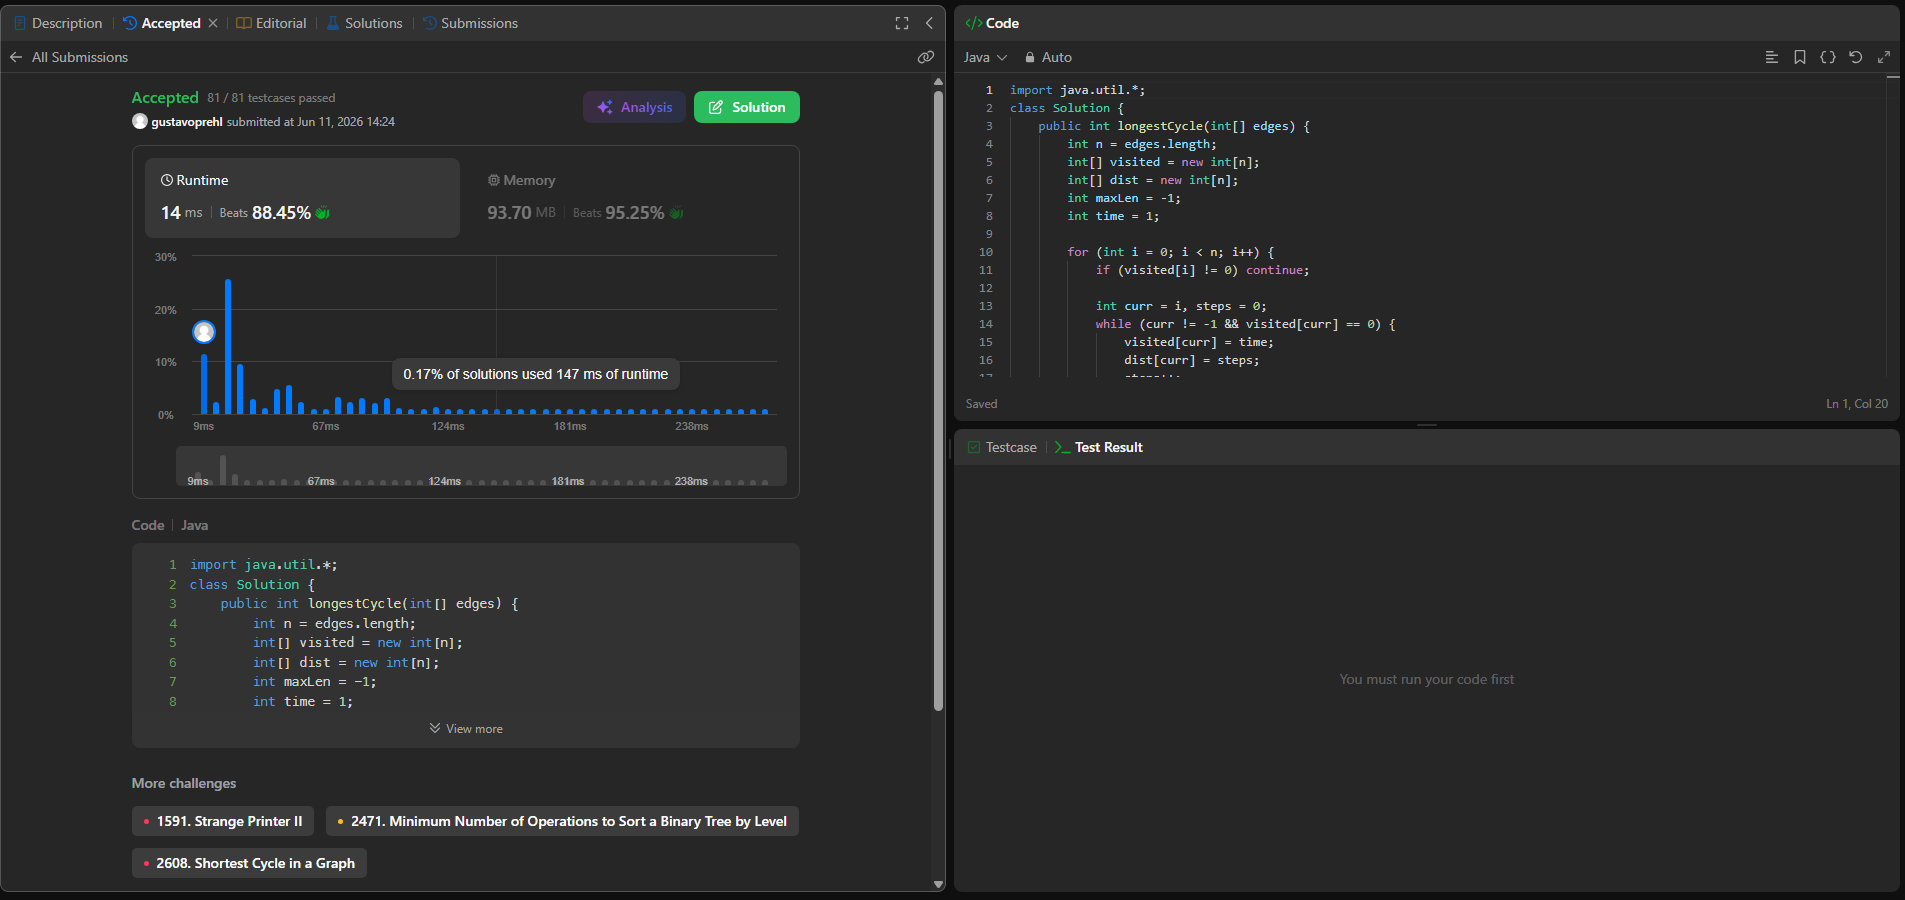
\includegraphics[width=0.85\textwidth]{Accepts/2360_LongestCycle_Submit.png}\\
\end{center}

\subsection*{Justificativa}

\textbf{Estratégia:} travessia iterativa de grafo funcional com marcação por
\emph{timestamp} (variação de busca em profundidade sem recursão/pilha
extra).

\textbf{Estrutura do problema:} como cada nó tem grau de saída no máximo 1, o
grafo é uma coleção de ``componentes funcionais'': cada um é uma cadeia de
nós que termina em $-1$ (sem ciclo) ou que eventualmente entra em um único
ciclo, em formato de $\rho$ (rho). Isso significa que, a partir de qualquer
nó, seguir os ponteiros \texttt{edges[i]} leva, no máximo, a um único ciclo.

\textbf{Algoritmo:} para cada nó \texttt{i} ainda não visitado, percorre-se a
cadeia a partir dele, atribuindo a cada nó visitado nessa travessia um
\texttt{timestamp} (identificador da travessia atual) e a sua distância
(\texttt{dist}, número de passos desde \texttt{i}). A travessia para quando:
\begin{itemize}
    \item chega a $-1$ (cadeia sem ciclo) --- não há ciclo a contabilizar; ou
    \item chega a um nó já visitado:
    \begin{itemize}
        \item se o \texttt{timestamp} desse nó for o \textbf{mesmo} da
        travessia atual, então o nó faz parte de um ciclo encontrado
        \textbf{agora}, e o tamanho do ciclo é
        \texttt{passos\_atuais - dist[nó]} (a diferença entre quando o nó
        foi ``reencontrado'' e quando foi visitado pela primeira vez nesta
        mesma travessia);
        \item se o \texttt{timestamp} for de uma travessia
        \textbf{anterior}, a cadeia atual apenas se conecta a um componente
        já processado, sem formar um novo ciclo.
    \end{itemize}
\end{itemize}

\textbf{Por que cada nó é processado uma única vez (correção da
complexidade):} uma vez que \texttt{visited[curr] != 0}, o nó nunca é
revisitado por outra travessia (a condição \texttt{visited[curr] == 0} no
laço \texttt{while} impede isso). Logo, cada nó é marcado e processado
exatamente uma vez ao longo de todas as travessias.

\textbf{Complexidade:}
\begin{itemize}
    \item Tempo: $O(n)$, pois cada nó é visitado uma única vez no total,
    somando todas as travessias.
    \item Espaço: $O(n)$ para os vetores \texttt{visited} e \texttt{dist}.
\end{itemize}

\textbf{Tópico do curso:} \emph{Análise de Algoritmos Iterativos} [CLRS09,
caps. 1 e 2.2] --- o algoritmo é estruturado como laços iterativos (sem
recursão), e o argumento de que cada nó é marcado e processado no máximo uma
vez é o que garante o limite $O(n)$ no total de iterações.
